%-----------------------------------------------------------------------------
%
%               Template for sigplanconf LaTeX Class
%
% Name:         sigplanconf-template.tex
%
% Purpose:      A template for sigplanconf.cls, which is a LaTeX 2e class
%               file for SIGPLAN conference proceedings.
%
% Guide:        Refer to "Author's Guide to the ACM SIGPLAN Class,"
%               sigplanconf-guide.pdf
%
% Author:       Paul C. Anagnostopoulos
%               Windfall Software
%               978 371-2316
%               paul@windfall.com
%
% Created:      15 February 2005
%
%-----------------------------------------------------------------------------


\documentclass[preprint,10pt]{sigplanconf}

% The following \documentclass options may be useful:

% preprint      Remove this option only once the paper is in final form.
% 10pt          To set in 10-point type instead of 9-point.
% 11pt          To set in 11-point type instead of 9-point.
% authoryear    To obtain author/year citation style instead of numeric.

\usepackage{amsmath}
\usepackage{graphicx}
\usepackage{listings}
\usepackage{color}

\definecolor{mygreen}{rgb}{0,0.6,0}

\lstset{language=Java} 

\lstset{ %
  breakatwhitespace=false,          % sets if automatic breaks should only happen at whitespace
  breaklines=true,                  % sets automatic line breaking
  commentstyle=\color{mygreen}, 
  captionpos=none,                  % sets the caption-position to bottom
  frame=single,                     % adds a frame around the code
  keepspaces=true,                  % keeps spaces in text
  language=Java,                    % the language of the code
  morekeywords={function,var},      % if you want to add more keywords to the set
  numbers=left,                     % where to put the line-numbers; possible values are (none, left, right)
  numbersep=5pt,                    % how far the line-numbers are from the code
  keywordstyle=\color{blue},
  %numberstyle=\tiny,               % the style that is used for the line-numbers
  showspaces=false,                 % show spaces everywhere adding particular underscores; it overrides 'showstringspaces'
  showstringspaces=false,           % underline spaces within strings only
  showtabs=false,                   % show tabs within strings adding particular underscores
  stepnumber=1,                     % the step between two line-numbers. If it's 1, each line will be numbered
  tabsize=2,                        % sets default tabsize to 2 spaces
  title=\lstname,                   % show the filename of files included with \lstinputlisting; also try caption instead of title
}

\lstdefinestyle{full}{
  frame=single,
  numbers=left,
  keepspaces=true,
  basicstyle=\footnotesize\ttfamily,
  belowcaptionskip=1\baselineskip,
  aboveskip=0.5cm,
  belowskip=0.5cm
}

\lstdefinestyle{tablecode}{
  frame=none,
  numbers=none,
  keepspaces=false,
  basicstyle=\footnotesize\ttfamily,
  belowcaptionskip=1\baselineskip,
  aboveskip=0cm,
  belowskip=0cm
}

\begin{document}

\special{papersize=8.5in,11in}
\setlength{\pdfpageheight}{\paperheight}
\setlength{\pdfpagewidth}{\paperwidth}

\conferenceinfo{OOPSLA '15}{October 25--30, 2015, Pittsburgh, Pennsylvania, United States} 
\copyrightyear{2015} 
\copyrightdata{978-1-nnnn-nnnn-n/yy/mm} 
\doi{nnnnnnn.nnnnnnn}

% Uncomment one of the following two, if you are not going for the 
% traditional copyright transfer agreement.

%\exclusivelicense                % ACM gets exclusive license to publish, 
                                  % you retain copyright

%\permissiontopublish             % ACM gets nonexclusive license to publish
                                  % (paid open-access papers, 
                                  % short abstracts)

\titlebanner{}        % These are ignored unless
\preprintfooter{Improving JavaScript performance through Source Code Rewriting}   % 'preprint' option specified.

\title{Optimizing JavaScript through Source Code Rewriting}
% \subtitle{Subtitle Text, if any}

% \authorinfo{Alexis Ferreyra}
           % {UTN-FRC}
           % {alexis.ferreyra@gmail.com}
% \authorinfo{Ricardo Medel}
           % {UTN-FRC}
           % {ricardo.medel@gmail.com}
% \authorinfo{Emanuel Ravera}
           % {UTN-FRC}
           % {emanuel.ravera@gmail.com}

%\authorinfo{Alexis Ferreyra \and Ricardo Medel \and Emanuel Ravera}
%           {Universidad Tecnologica Nacional - Facultad Regional Cordoba}
%           {alexis.ferreyra@gmail.com \and ricardo.medel@gmail.com}

\authorinfo {Authors omitted for submission}
            {}
            {}

\maketitle

\begin{abstract}
The expansion of the World Wide Web, and web runtimes in particular, to all kind of devices has render the JavaScript performance in a hot topic in recent years. Several approaches to improve the performance of JavaScript applications have been tried by the industry and research community. In this paper we review the most popular approaches and propose a novel solution based on meta-programming and code rewriting. The preliminary results of our experiments are very promising, although more studies are required to know to what extent our approaches can improve the performance of real-life JavaScript programs.
\end{abstract}

\category{D.3.4}{Programming Languages}{Processors}[Code generation]

% general terms are not compulsory anymore, 
% you may leave them out
% \terms
% term1, term2

\keywords
Performance, Meta-programming, Macros, Rewriting, JavaScript, Compiler

\section{Introduction}
Improving JavaScript performance have been a hot topic in the recent years. The ubiquity of the World Wide Web, and web runtimes in particular, across all kind of devices in addition to an always increasing complexity of applications written in JavaScript have drawn attention of the industry and research community towards the improvement of JavaScript performance and security.

In this paper we focus on the performance aspects of this problem, reviewing the most popular approaches, proposing a novel solution based on meta-programming and code rewriting, and showing the preliminary results of our experiments.

Most of the work to boost the performance of programs written in JavaScript is focused on improving compiler/execution infrastructure, such as the Safari SquirrelFish runtime [10], the just in time (JIT) compiler Google V8 [7], or the work done by the Mozilla team on trace based optimizations [9]. Other approaches are also being tried. Mozilla asm.js [1] is a subset of JavaScript for which highly efficient code can be generated on the fly, while Intel is trying to add new extensions to the language, like SIMD [11] instructions or support for parallel execution [16] of certain APIs.

Our work explored the feasibility of improving performance at a higher level by using code rewriting at compile time, well before the source code reaches the JavaScript runtime. We found several cases where JavaScript performance is highly sensitive to the way in which the programmer writes the code. For example, as we show in Section \ref{sec:benchmarks}, using the \emph{`for in'} statement to iterate an array object is at least 25 times slower than using a standard \emph{`C style for'} to iterate the same array. Even more remarkable, different APIs generating the same or semantically similar results can show a bigger difference in run times. For example, using the API \emph{`document.getElementByTagName'} to find elements in the DOM can be 200 times faster than using the API \emph{`document.querySelectorAll'}  to retrieve elements by tag name.

The proposal is to improve the performance of JavaScript programs by analysing this type of cases, which are out of reach of JIT compilers and runtimes, with program introspection and rewriting techniques. To test our hypothesis we identified a number of patterns to be optimized, and then implemented synthetic benchmarks to check if replacing slow patterns with the fast ones provides measurable performance benefits. Once we checked that these patterns actually generate sizable improvements in the synthetic benchmarks, we designed and implemented a general tool to easily automate the desired refactoring. The tool, named PumaScript, is a simple JavaScript dialect extended with program introspection and rewriting capabilities. Finally, by using PumaScript we implemented meta-functions to automatically rewrite code that runs slow with faster, semantically equivalent code.

\section{JavaScript Patterns and Benchmarks}
\label{sec:benchmarks}
In this section we compare the performance of several patterns with code with similar semantics but faster execution time, and we also propose a solution for the cases where the semantics is not exactly the same.

During our exploration, we identified five JavaScript patterns, showed in Table 1, which can be written in more than one way and still achieve the same result. The first column of the table describes the pattern, the second column shows the original code and the third shows code that is semantically equivalent but it can run faster.

\lstset{style=tablecode}

\begin{table*}
\begin{tabular}{ |  l  |  p{3.2cm} | p{6.1cm} | p{6.5cm} | }
\hline
N & 
Description & 
Original Code & 
Improved Code \\
\hline
1 &
Iterate an array using “For In” vs “C For” statements &
\begin{lstlisting}
var array = [1,2,3 ...];

for (var i in array) {
  array[i] +=1;
} 
\end{lstlisting} 
&
\begin{lstlisting}
var array = [1,2,3 ...];
for (var i=0; i< array.length; i++) {
  array[i] +=1;
}
\end{lstlisting}
\\
\hline
2 &
Native selector by ID vs jQuery ID selector &
\begin{lstlisting}
$("#test");
\end{lstlisting}
&
\begin{lstlisting}
$(document.getElementById("test"));
\end{lstlisting}
\\
\hline
3 &
Round an integer using parseInt vs bitwise operator &
\begin{lstlisting}
var number = Math.random() * 1000;
parseInt(number);
\end{lstlisting}
&
\begin{lstlisting}
var number = Math.random() * 1000;
number | 0;
\end{lstlisting}
\\
\hline
4 &
querySelectorAll vs. getElementsByClassName &
\begin{lstlisting}
var items = document.querySelectorAll(".test");
\end{lstlisting}
&
\begin{lstlisting}
var item = document.getElementsByClassName("test");
\end{lstlisting}
\\
\hline
5 &
querySelectorAll vs. getElementsByTagName &
\begin{lstlisting}
var items = document.querySelectorAll("test");
\end{lstlisting}
&
\begin{lstlisting}
var items = document.getElementsByTagName("test");
\end{lstlisting}
\\
\hline
\end{tabular}
\caption{JavaScript patterns in their original and improved form.}
\label{tab:1}
\end{table*}

After identifying the JavaScript patterns, we created and run synthetic benchmarks for each of them in order to measure the difference in performance between the original version of the pattern and the improved one. Table 2 shows the observed performance improvements for the JavaScript patterns when run on different hardware and browsers. As the table shows, we run the benchmarks across two desktop browsers and two Android browsers. 
The hardware used to run desktop browsers was one notebook Lenovo T430, 4GB RAM, dual core processor Intel Core i5-3320M 2.60Hz with Windows 8 operating system. For benchmarking Android browsers a Tablet Asus MeMO Pad 7 with an Intel Atom Z3560 1.83GHz quad core processor, 2GB RAM and Android 4.4.2.

\begin{table}
\begin{tabular}{ |  l  |  r | r | r | r | }
\hline
N & 
\parbox[t]{1.5cm}{PC Chrome v36} &
\parbox[t]{1.5cm}{PC Mozilla v30} &
\parbox[t]{1.5cm}{Android Tablet Native Browser} &
\parbox[t]{1.5cm}{Android Tablet Chrome v36} \\
\hline
1 &
55.54x &
167.60x &
27.96x &
25.26x \\
\hline
2 &
2.15x &
1.49x &
1.98x &
1.79x \\
\hline
3 &
12.91x &
33.30x &
11.24x &
4.75x \\
\hline
4 &
138.88x &
364.97x &
915.23x &
394.26x \\
\hline
5 &
236.16x &
393.29x &
213.69x &
146.89x \\
\hline
\end{tabular}
\caption{Improvement rate for each pattern comparing slow and fast forms.}
\label{tab:2}
\end{table}

As it can be seen in the table, the improvement in performance between the slower and the fastest version of a pattern ranges between 1.49 times for the worst case (pattern 2 on a desktop PC with a Mozilla browser) and up to 915.23x times for the best case (pattern 4 on an Android tablet).

\subsection{Solving Semantic Differences}
Notice, however, that patterns 4 and 5 are optimistic transformations, since the original and improved code will generate the same result most of the time, but not always. This discrepancy exists because the \emph{querySelectorAll} method returns an instance of a \emph{NodeList} object, while \emph{getElementsByClassName} and \emph{getElementsByTagName} return an \emph{HTMLCollection} object. Both objects, \emph{NodeList} and \emph{HTMLCollection} are similar, since both are collections containing the properties \emph{length} and \emph{item()}, which are used to get the number of items in the collection and to get an specific item, respectively. But because both collections use different constructors, a code that checks for the instance type of the collection can fail in the translated version. Other consideration to take in account is that \emph{HTMLCollection} objects are live collections, this means that when the DOM is updated the collection is updated. For example, after retrieving all nodes with class name `class1' by using the \emph{getElementsByClassName} method, if a new node with `class1' class name is added to the DOM, the collection will be automatically updated.

Although for most cases the differences between \emph{HTMLCollection} and \emph{NodeList} will not change the semantic of the program, it may be the case. Fortunately, there is a way to circumvent this semantic difference between the two collection types. When rewriting calls to \emph{querySelectorAll} into calls to \emph{getElementsByClassName} or \emph{getElementsByTagName} it is possible to wrap the returned collection with a new \emph{NodeList} collection. Table 3 shows the original and the improved code for this two patterns. Figure 1 shows the method \emph{createNodeList}, which converts an \emph{HTMLCollection} object into a \emph{NodeList} collection.

\lstset{style=full}

\begin{figure}
\begin{lstlisting}
function createNodeList (elements) {
    var fragment = document.createDocumentFragment();
    for(var i; i < elements.length; i++)
        fragment.appendChild(elements[i]);
    return fragment.childNodes;
};
\end{lstlisting}
\caption{Helper function to convert from HTMLCollection into NodeList.}
\label{fig:1}
\end{figure}

After applying these changes for patterns 4 and 5 and running the benchmarks again, it was found that the improvement in a PC using Chrome was down from 138.88 times faster to a more conservative 17.2 times faster. Still, this is a sizable improvement in performance between using \emph{querySelectorAll} and \emph{getElementsBy...} methods.

\section{Implementing a Meta-Programming and Rewriting Infrastructure}
In order to automate the process of rewriting the identified patterns, and also as a way to have a general framework to experiment with code introspection and meta-programming applied to improving language performance, a new JavaScript dialect and rewriting infrastructure were designed and implemented. We created PumaScript, a superset of JavaScript which main new feature is the support for meta-functions. This mechanism works in a similar way to programmable macro-expansion systems as the ones available in Lisp and other programming languages. 

Like other macro systems, PumaScript meta-functions can expand caller expressions inline. A meta-function takes the decorated syntax tree (AST) of the declared parameters as actual arguments and returns the target AST to be used as a replacement for the caller expression. However, there are two big differences between PumaScript meta-functions and other macro systems: 

\begin{enumerate}
  \item A PumaScript meta-function can decide to not expand a certain occurrence of a caller expression by returning a `null' value instead of an AST.
  \item PumaScript does not have a special `macro-expansion' phase before fully executing the program. Instead, meta-functions are live functions just like normal functions and can be called any time in the lifetime of the program.
\end{enumerate}
  
Our meta-functions can execute any arbitrary computation, including calling other normal functions or meta-functions. Additionally, all meta-functions have access to special intrinsic functions which provides access for introspection and re-writing of any portion of the program’s syntax tree. 

As a simple example of a PumaScript meta-function, the Figure 2 shows a meta-function that rewrites a simple call into a simple addition expression.

\begin{figure}
\begin{lstlisting}
/** @meta */ 
function sum(a, b)
{
    return pumaAst( $a +  $b);
}

// this call will be expanded 
// to “5 + 6” expression
sum(5, 6); 
\end{lstlisting}
\caption{A simple meta function and its invocation.}
\label{fig:2}
\end{figure}

The current high level implementation and execution process of PumaScript is shown in Figure 3. We use the Esprima [19] library to parse the JavaScript-like syntax. Then the PumaScript runtime is used to execute the Abstract Syntax Tree following the standard JavaScript semantic plus the additional rules and semantics added by PumaScript. Once the program is executed, PumaScript runtime discards the meta-functions nodes and the resulting Decorated Syntax Tree is processed by the Escodegen [13] library in order to pretty print the program into standard JavaScript.

\begin{figure*}
\begin{center}
	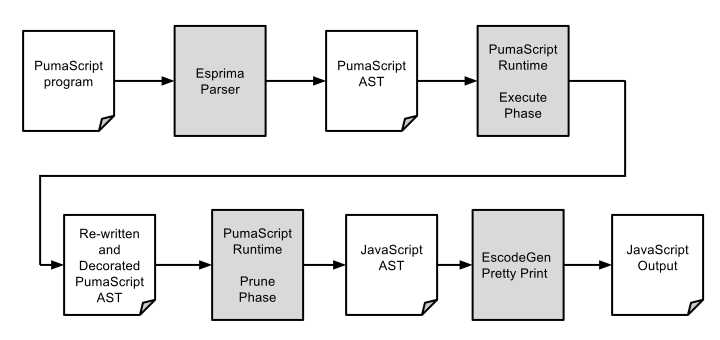
\includegraphics[width=1\textwidth]{puma-stack}
\end{center}
\caption{PumaScript program execution workflow and high level modules.}
\label{fig:3}
\end{figure*}

\subsection{PumaScript Meta-Functions}
As seen in Figure 2, PumaScript meta-functions are written just like normal JavaScipt functions and adding the annotation @meta in a comment before the function declaration. This method is used to avoid introducing a new syntax requirement, making PumaScript backward compatible with standard JavaScript.

Meta-functions work in a similar way than regular JavaScript functions, with three specific differences:

\begin{enumerate}
  \item All parameters in a meta-function will evaluate to a reference into the caller argument Decorated Syntax Tree at the moment of execution. 
For example, when calling the meta-function ``foo(a, b)'' with actual argument expressions ``2 * x'' and ``3 * y'' respectively for parameters ``a'' and ``b''; the parameter ``a'' will take the value of the syntax tree for ``2 * x'' and the parameter ``b'' will take the value of the syntax tree ``3 * y''.
  \item All meta-functions must return a valid syntax tree or null. If the return value is null, then the caller expression will not be rewritten. Otherwise, If the return value is a non-null syntax tree, the caller expression will be replaced with the returned syntax tree, actually rewriting the caller expression in the process.
  \item All meta-functions have access to a reserved context with intrinsic objects and functions that can be used to make introspection into the program or to rewrite any portion of the program. Sample intrinsic objects and functions available in the meta-function context are: \emph{pumaAst}, \emph{context} or \emph{pumaFindByType}.
\end{enumerate}

Figure 4 shows a simple PumaScript program and its output. In this example the meta-function \emph{firstLetter} rewrites its callers if the actual argument is a string literal. Otherwise, the function returns null and avoids rewriting the caller expression.

\begin{figure}
\begin{lstlisting}
// Program sent to PumaScript

/** @meta */ 
function firstLetter(valueExp){
    var ast = null;
    if(valueExp.type === "Literal"){
        ast = valueExp;
        ast.value = ast.value.substring(0, 1);
    }
    return ast;
}

// this call will be rewritten to "H";
firstLetter("Hello World"); 

// this call will not be rewritten 
// because the argument expression is not a literal
firstLetter("Hello " + "World");

// Output of PumaScript
"H";
firstLetter("Hello " + "World");
\end{lstlisting}
\caption{A meta-function replacing string literals and its invocation.}
\label{fig:4}
\end{figure}

Figure 5 shows a PumaScript meta-function that counts all the occurrences of \emph{for} statements in a script and outputs the number by using the standard console object. In this example the function \emph{pumaFindByType} and the object \emph{pumaProgram} are intrinsic objects available in the context of any meta-function. These objects and functions can be used to introspect any portion of the program not only the current context which is calling the meta-function.

\begin{figure}
\begin{lstlisting}
/** @meta */
function countForStatemets() {
    var forStas = pumaFindByType(pumaProgram, "ForStatement");
    console.log("For statements found: " + forStas.length);
    return null;
}
\end{lstlisting}
\caption{Meta-function counting the number of “for” statements in a program.}
\label{fig:5}
\end{figure}

\subsection{Rewriting Code to Make It Performant}
In this section we describe how automatic rewriting of patterns were implemented using our PumaScript language. First, we introduce and explain the code used to rewrite the JavaScript pattern 2, previously introduced in Table \ref{tab:1}, which translate jQuery selectors into a native JavaScript API call. Then, we discuss the implementation used to implement the rewriting of pattern 1 to transform \emph{for-in} statements into the more efficient \emph{C style for} statements.

\subsubsection{Rewrite jQuery Selector Calls}
Figure 6 shows a meta-function that rewrites jQuery selectors by Id into the more efficient native API \emph{`document.getElementById'}. Line 6 checks that the actual argument is a Literal node and tests for the regular expression used to match selectors by Id. Then, it removes the `\#' character from the beginning and returns a new syntax tree (AST) using \emph{`document.getElementById'} and the provided argument with the modified string literal. The intrinsic function \emph{pumaAst} is used to build the returned AST, starting from a template where the local variables are expanded with their actual values.

\begin{figure}
\begin{lstlisting}
/* @meta */
function $(valueExp){
  var regex = /^#\b[a-zA-Z0-9_]+\b$/;
  var argValue = {};
  
  if(valueExp.type === "Literal" && regex.test(valueExp.value)){
    valueExp.value = valueExp.value.substring(1);
    return pumaAst($(document.getElementById($valueExp)));   
  } 
  else if(OPTIMISTIC_REWRITE){
    argValue = evalPumaAst(valueExp).value;   
    if(regex.test(argValue)){
      console.log("WARNING: Optimistic rewrite at line(" + valueExp.loc.start.line + ")");
      return pumaAst($(document.getElementById($valueExp.substring(1))));
    }
  }
  return null;
}
\end{lstlisting}
\caption{Meta function to rewrite jQuery selectors by Id.}
\label{fig:6}
\end{figure}

The simplest use case happens when the meta-function is called with a simple string literal argument. 

\begin{lstlisting}
// invocation with literal
var myElement = $("#Element_Id_1");
\end{lstlisting}

In this case, it is always safe to rewrite the invocation and the execution of the meta-function of Figure 6 will follow the \emph{then} branch of the \emph{if-else} statement of line 6.

On the other hand, when the actual argument to the meta-function is not a simple literal, the meta-function can use the intrinsic function \emph{evalPumaAst} to evaluate any portion of AST in the current execution context. 

The meta-function of Figure 6 uses a flag variable \emph{OPTIMISTIC\_REWRITE} to enable optimistic rewriting when it can check that at least one execution of the caller expression matches the selector by Id form. The following invocation may not be safe to rewrite if the variable \emph{element\_id} is an argument into a function, but by using the \emph{evalPumaAst} intrinsic function in line 11, the meta-function is able of detect that the call is safe to rewrite into a more efficient API call.

\begin{lstlisting}
// invocation with non-trivial expression
var element_id = "5";
var myOtherElement = $("#Element_Id_" + element_id);
\end{lstlisting}

Finally, there are cases where the selector do not match a simple selector by Id. 

\begin{lstlisting}
// invocation that does not match a selector by Id
var myOtherClassElements = $(".Class_Id_" + element_id);
\end{lstlisting}

The meta-function is capable of identifying this case easily, because no matter what value the variable \emph{element\_id} takes, it will not form a valid selector by Id.

\subsubsection{Rewrite \emph{for-in} Statements}
In order to implement the automatic rewriting of \emph{for-in} statements into \emph{C style for} statements, a different approach is needed. It is not possible to use a meta-function like a macro call which rewrites the caller expression. Instead, the meta-function to rewrite \emph{for-in} sentences needs to use intrinsic functions provided by the PumaScript runtime environment to introspect the AST of the running program.

Figure 7 shows the main meta-function used to rewrite \emph{for-in} statements. In line 5, it uses the intrinsic function \emph{pumaFindByType} and the intrinsic object \emph{pumaProgram} to match all AST nodes whose type is \emph{ForInStatement}. Then, the function iterates this list and uses a helper function to rewrite each \emph{for-in} subtree.

\begin{figure}
\begin{lstlisting}
/** 
 * @meta
 */
function rewriteForIn() {
  var forIns = pumaFindByType(pumaProgram, "ForInStatement");
  console.log("For In statements found: " + forIns.length);
  
  for(var index = 0; index < forIns.length; index++)
  {
    rewriteSingleForIn(forIns[index]);
  }
  return null;	
}
\end{lstlisting}
\caption{Main meta-function to rewrite \emph{for-in} statements}
\label{fig:7}
\end{figure}

The helper function to rewrite a single \emph{for-in} sentences has 4 main steps:
\begin{enumerate}
  \item To detect if the \emph{for-in} statement uses a variable declaration as the iteration reference or if it reuses an existing variable for the iteration reference.
  \item To create a new AST for an equivalent \emph{C style for} sentence.
  \item To create an \emph{if} statement that will be used as type guard to fallback into the original \emph{for-in} if the type of the collection expression to be iterated is not an array.
  \item To replace the original \emph{for-in} AST node with the generated \emph{if} AST node.
\end{enumerate}

Figure 8 shows the code implementing this behaviour. Note that the function is not marked as a meta-function, as PumaScript can arbitrarily mix meta-functions with normal functions.

\begin{figure}
\begin{lstlisting}
function rewriteSingleForIn(forInAst){
  var left = forInAst.left;
  var right = forInAst.right;
  var itemName;
  var tempId;
  
  // detect which kind of iteration variable it uses
  if(left.type === "Identifier")
  {
    itemName = left;
  }
  else if(left.type === "VariableDeclaration")
  {
    tempId = left.declarations[0].id;
    itemName = pumaAst( $tempId );
  }
  else
  {
    return;
  }

  // prepare fallback version and optimized AST
  var cloneForIn = pumaCloneAst(forInAst);
  var optimizedFor = pumaCloneAst(forInAst);

  optimizedFor.type = "ForStatement";
  optimizedFor.init = left;
  optimizedFor.test = pumaAst( $itemName < $right.length );
  optimizedFor.update = pumaAst( $itemName = $itemName + 1 );
  
  // create type-guard to test runtime type
  var temp = pumaAst(function(){
    if( Array.isArray( $right ) ) $optimizedFor; else $cloneForIn;
  });
  var tempIf = pumaFindByType( temp, "IfStatement")[0];

  // replace original node with type-guard one
  forInAst.type = tempIf.type;
  forInAst.test = tempIf.test;
  forInAst.consequent = tempIf.consequent;
  forInAst.alternate = tempIf.alternate;
}
\end{lstlisting}
\caption{Helper function to rewrite single \emph{for-in} statement.}
\label{fig:8}
\end{figure}

Having the code to rewrite \emph{for-in} into \emph{C style for} available, Figure 9 shows a sample client program that calls the meta-function to rewrite \emph{for-in} statements. The output obtained from running this program is shown in Figure 10.

\begin{figure}
\begin{lstlisting}
var array = [1,2,3,4,5,6,7,8,9,0];
var i = 0;

// test for-in with existing iteration variable
for(i in array){
  array[i] += 1;
}

// test for-in with new iteration variable
for(var j in array){
  array[j] += 1;
}

// call to meta-function to optimize for-in
rewriteForIn();
\end{lstlisting}
\caption{Sample client program which uses the \emph{rewriteForIn} meta-function.}
\label{fig:9}
\end{figure}

% Finally, the output of running this program is shown in Figure 10.
% As the figure shows, optimized versions of the original \emph{for-in} are generated  in addition to an if-statement which is used as a type-guard to check that % the collection expression is actually an array at runtime. With further static analysis techniques, this type-guard maybe removed when if the meta-function which perform the rewrite can calculate that the type of the collection expression is always an array.

\begin{figure}
\begin{lstlisting}
var array = [1, 2, 3, 4, 5, 6, 7, 8, 9, 0];
var i = 0;

if (Array.isArray(array))
  for (i; i < array.length; i = i + 1) {
    array[i] += 1;
  }
else
  for (i in array) {
    array[i] += 1;
  }
  
if (Array.isArray(array))
  for (var j; j < array.length; j = j + 1) {
    array[j] += 1;
  }
else
  for (var j in array) {
    array[j] += 1;
  }
\end{lstlisting}
\caption{Output generated by PumaScript after running program in Figure 9.}
\label{fig:10}
\end{figure}


\section{Related Work}
To our knowledge, source-to-source code rewriting techniques were never before used to improve JavaScript performance. Still, as previously established, there are several approaches to improve the performance of JavaScript programs. In this section we review other source code rewriting tools, then we describe commonly used JavaScript preprocessing tools, and finally we analyze the most relevant approaches to improve performance and compare them with our proposal.

\subsection{Rewriting and Preprocessing Tools}

\subsubsection{Source Code Rewriting Frameworks}

A number of frameworks and tool chains does exists which can be used to implement end-to-end source code cross-compilation or refactoring. Stratego XT [17] and DMS [18] are two of the more developed frameworks to build source-to-source transformation tools by using rewriting techniques. The main strength of these frameworks is their flexibility. They provide end-to-end tools to build parsers, rewriting scripts, semantic analyzers, and pretty printers. Our approach, as implemented by PumaScript, is simpler and does not aim to be a generic tool to transform from any source to any possible target. We focus in JavaScript language rewriting. 

Moreover, building and end-to-end JavaScript-to-JavaScript tool with these frameworks requires an important amount of work because every major component must be created using these tools. In contrast, in the implementation of PumaScript we reuse existing and tested components like the Esprima [19] parser for the front-end and EscodeGen [13] for pretty printing.

Another major difference between these frameworks and our solution, is that to implement transformations in these frameworks the developer must learn specific languages based on the tree rewriting paradigm. This programming paradigm is not well known by most developers. Instead, PumaScript meta-functions use the same JavaScript programming language that any JavaScript developer already knows. Our approach does not introduce a significantly new programming paradigm beyond requiring familiarity with macro-expansion systems, which are already available in a number of well known programming languages, such as Lisp or Ruby.

\subsubsection{Code Minifiers and Pre-Compilers}

Code minifiers have been utilized by JavaScript community for a long time. Simple minifiers like JSMin [2] and JSZap [3] provide mostly bandwidth optimization but not measurable performance improvements.
Elaborated precompilers like Google Closure Compiler [6] are capable of more advanced optimizations like code inlining and removing unused variables. But those optimizations are provided as a mean to shorten the source code and not as a way to improve performance.

\subsection{JavaScript Performance Improvement Approaches}

\subsubsection{Runtimes and Just in Time Compilers}

The greater performance improvement in JavaScript language has been related with the progression from using runtimes, like Safari SquirrelFish [10], to more advanced JIT compilers, such as Chrome V8 [7], Mozilla SpiderMonkey [9] or Microsoft Chakra [14]. 

All of these JIT-based engines reuse techniques previously used in other language runtimes, most notably the Java HotSpot compiler [15]. Although the introduction of JIT compilers has provided an improvement of at least one order of magnitude, even the more advanced JIT engines cannot optimize certain language patterns, such as \emph{for-in} vs \emph{C style for}. Also, JIT engines are not good candidates to incorporate optimizations related to similar APIs with different performance, like the cases for jQuery selectors vs. native APIs identified in this work.

\subsubsection{Language Extensions}

Language extensions like Mozilla asm.js [1] or Intel proposed SIMD [11] and parallel execution [16] extensions are capable of providing important performance benefits for certain use cases. But these approaches suffer from several limitations. First, developers must embrace the language extensions by using them in their source code. Second, runtime providers must implement the support for these extensions in their runtimes. These limitations generate the classic chicken-and-egg problem: developers are not willing to invest effort in modifying their code until most runtime providers add support for a certain language extension, while at the same time, runtime providers are not encouraged to support the extensions because there are not big amounts of source code in the wild which use them.

In contrast, our approach can be used from day one by developers, not requiring them to change the source code and having immediate benefits in existing runtimes. The only additional cost for a developer to use our method, is to add PumaScript and the rewriting scripts to her deployment process.

\section{Summary and Future Work}
In this work we show that the performance of JavaScript programs is highly sensitive to a number of source code and API patterns, and thus sizable performance improvements can be achieved by replacing these patterns by the corresponding faster code.

Also, we introduce a JavaScript language extension called PumaScript, which can be used to automate a number of source code rewriting tasks. This new framework adds to JavaScript a novel kind of functions which can introspect and rewrite syntax trees on the fly,  without requiring the program to be restarted or a specific macro-expansion phase in the runtime.

By using PumaScript, we demonstrated that it is possible to automate the source code rewriting needed to convert slow JavaScript patterns into faster ones. Then, developers can integrate PumaScript rewriting infrastructure and transformation scripts into their continuous integration environments to optimize the source code before deploying. Additionally, our novel approach to improve performance is complementary to progress in JavaScript runtimes, high performance language subsets and other efforts to improve the language performance.

Still, there is additional work to be done in order to validate how the exhibited performance benefits of rewriting non-optimal patterns in our synthetic benchmarks translate to real life code. The first open question is to analyze how common these non-optimal patterns are in actual JavaScript source code. Moreover, it is possible that several other non-optimal patterns exist and can benefit from our approach.

Finally, we would like to explore the use of our PumaScript infrastructure in other applications related to JavaScript meta-programming. For example, it could be applied to source code generation, construction of static, precompiled domain specific languages, static and realtime source code analysis, application of aspect oriented programming, source code instrumentation, and source-to-source transformation to other scripting languages.


%\appendix
%\section{Appendix Title}

%This is the text of the appendix, if you need one.

%\acks

%Acknowledgments, if needed.

% We recommend abbrvnat bibliography style.

\bibliographystyle{abbrvnat}

% The bibliography should be embedded for final submission.

\begin{thebibliography}{}
\softraggedright

%\bibitem[Smith et~al.(2009)Smith, Jones]{smith02}
%P. Q. Smith, and X. Y. Jones. ...reference text...

\bibitem{} David Herman, Luke Wagner, and Alon Zakai. asm.js specification. http://asmjs.org/spec/latest/, 2013.

\bibitem{} D. Crockford. JSMin: The JavaScript minifier. http://www.crockford.com/javascript/jsmin.html.

\bibitem{} Martin Burtscher , Benjamin Livshits , Benjamin G. Zorn , Gaurav Sinha, JSZap: compressing JavaScript code, Proceedings of the 2010 USENIX conference on Web application development, p.4-4, June 23-24, 2010, Boston, MA

\bibitem{} Paruj Ratanaworabhan , Benjamin Livshits , Benjamin G. Zorn, JSMeter: comparing the behavior of JavaScript benchmarks with real web applications, Proceedings of the 2010 USENIX conference on Web application development, p.3-3, June 23-24, 2010, Boston, MA

\bibitem{} Mason Chang , Edwin Smith , Rick Reitmaier , Michael Bebenita , Andreas Gal , Christian Wimmer , Brendan Eich , Michael Franz, Tracing for web 3.0: trace compilation for the next generation web applications, Proceedings of the 2009 ACM SIGPLAN/SIGOPS international conference on Virtual execution environments, March 11-13, 2009, Washington, DC, USA

\bibitem{} Google closure compiler. https://developers.google.com/closure/compiler.

\bibitem{} v8. Google Inc. V8 JavaScript virtual machine. https://code.google.com/p/v8, 2013.

\bibitem{} Brian Hackett , Shu-yu Guo, Fast and precise hybrid type inference for JavaScript, Proceedings of the 33rd ACM SIGPLAN conference on Programming Language Design and Implementation, June 11-16, 2012, Beijing, China

\bibitem{} A. Gal, B. Eich, M. Shaver, D. Anderson, B. Kaplan. G. Hoare, D. Mandelin, B. Zbarsky, J. Orendorff, J. Ruderman, E. Smith, R. Reitmaier, M. R. Haghighat, M. Bebenita, M. Chang, and M Franz; ``Trace-based Just-in-Time Type Specialization for Dynamic Languages;'' in Programming Language Design and Implementation (PLDI 2009), Dublin, Ireland; June 2009

\bibitem{} Surfin’ Safari - Blog Archive - Announcing SquirrelFish - https://www.webkit.org/blog/189/announcing-squirrelfish/

\bibitem{} SIMD in JavaScript - Intel Corporation - https://01.org/node/1495

\bibitem{} Stephan Herhut , Richard L. Hudson , Tatiana Shpeisman , Jaswanth Sreeram, River trail: a path to parallelism in JavaScript, Proceedings of the 2013 ACM SIGPLAN international conference on Object oriented programming systems languages \& applications, October 29-31, 2013, Indianapolis, Indiana, USA

\bibitem{} ECMAScript code generator EscodeGen. https://github.com/estools/escodegen

\bibitem{} Advances in JavaScript Performance in IE10 and Windows 8 - http://blogs.msdn.com/b/ie/archive/2012/06/13/advances-in-javascript-performance-in-ie10-and-windows-8.aspx

\bibitem{} Michael Paleczny , Christopher Vick , Cliff Click, The java hotspotTM server compiler, Proceedings of the 2001 Symposium on JavaTM Virtual Machine Research and Technology Symposium, p.1-1, April 23-24, 2001, Monterey, California

\bibitem{} Stephan Herhut , Richard L. Hudson , Tatiana Shpeisman , Jaswanth Sreeram, River trail: a path to parallelism in JavaScript, ACM SIGPLAN Notices, v.48 n.10, October 2013

\bibitem{} M. Bravenboer, K. T. Kalleberg, R. Vermaas, and E. Visser. Stratego/XT 0.17. A Language and Toolset for Program Transformation. Science of Computer Programming, 72(1-2):52--70, June 2008.

\bibitem{} I. D. Baxter, C. Pidgeon, and M. Mehlich. DMS: Program transformations for practical scalable software evolution. In ICSE ’04: Proceedings of the 26th International Conference on Software Engineering, pages 625–634, Washington, DC, USA, 2004. IEEE Computer Society.

\bibitem{} ECMAScript parsing infrastructure for multipurpose analysis. http://esprima.org/

\end{thebibliography}


\end{document}

%                       Revision History
%                       -------- -------
%  Date         Person  Ver.    Change
%  ----         ------  ----    ------

%  2013.06.29   TU      0.1--4  comments on permission/copyright notices

